\chapter{Mecanismos de reação: etapas elementares e aproximações}\label{ch:b1:elementary-steps}

O monóxido de nitrogênio, formado nos motores dos carros e nos raios,
combina-se com o oxigênio do ar: \ce{2NO + O2 -> 2NO2}. Medida em
laboratório, a velocidade dessa reação é proporcional a
$[\ce{NO}]^2[\ce{O2}]$ --- e ela fica \emph{mais lenta} quando o gás é
aquecido. Uma única colisão de três moléculas poderia explicar o
primeiro fato, nunca o segundo: toda colisão fica mais energética com a
temperatura. A explicação é que a reação não é um evento único, mas uma
sequência de eventos mais simples, o seu mecanismo. Este capítulo define
essas \omterm{def:b1:elementary-steps:elementary-step}{etapas elementares}, o \omterm{def:b1:elementary-steps:energy-profile}{perfil de energia} ao longo do qual elas
ocorrem e as aproximações que transformam um mecanismo em uma \omterm{def:b1:rate-laws:order}{lei de
velocidade}; ele termina com a catálise, a arte de abrir um caminho mais
fácil.

\begin{recall}
O Livro 1 (ano 12) descreveu um \omterm{def:b1:elementary-steps:elementary-step}{mecanismo de reação} como uma sequência
de etapas desenhadas com setas curvas, com intermediários formados e
consumidos, e um \omterm{def:b1:elementary-steps:catalyst}{catalisador} como uma espécie que acelera uma reação sem
ser consumida. As \omterm{def:b1:rate-laws:order}{leis de velocidade}, as ordens e a \omterm{thm:b1:rate-laws:arrhenius}{lei de Arrhenius}
foram definidas no \cref{ch:b1:rate-laws}.
\end{recall}

\section{Etapas elementares}

\begin{definition}[Etapa elementar, molecularidade, mecanismo]\label{def:b1:elementary-steps:elementary-step}
Uma \emph{etapa elementar}\index{etapa elementar} é uma reação que ocorre
em um único evento molecular, tal como está escrita, sem nenhum
intermediário. Sua \emph{molecularidade}\index{molecularidade} é o número
de partículas que reagem nesse evento: 1 (unimolecular, uma decomposição
ou um rearranjo), 2 (bimolecular, uma colisão), raramente 3. Um
\emph{mecanismo de reação}\index{mecanismo de reacao@mecanismo de reação} é o conjunto das etapas
elementares cuja soma é a reação global. Uma espécie formada em uma
etapa e consumida em uma etapa posterior, ausente da equação global, é
um \emph{intermediário de reação}\index{intermediario de reacao@intermediário de reação}.
\end{definition}

\begin{proposition}[Lei de velocidade de uma etapa elementar]\label{prop:b1:elementary-steps:elementary-law}
Uma \omterm{def:b1:elementary-steps:elementary-step}{etapa elementar} admite uma ordem, e suas \omterm{def:b1:rate-laws:order}{ordens parciais} são iguais
a seus coeficientes estequiométricos: $\mathrm{A} \to \dots$ tem $v = k[\mathrm{A}]$;
$\mathrm{A} + \mathrm{B} \to \dots$ tem $v = k[\mathrm{A}][\mathrm{B}]$;
$2\,\mathrm{A} \to \dots$ tem $v = k[\mathrm{A}]^2$. A recíproca é falsa:
uma reação cujas ordens são iguais a seus coeficientes não é
necessariamente elementar.
\end{proposition}

\begin{proof}[Raciocínio]
Uma etapa bimolecular ocorre quando um \ce{A} encontra um \ce{B}; o
número desses encontros por unidade de volume e de tempo é proporcional
ao número de \ce{A} por unidade de volume e ao número de \ce{B}, logo a
$[\ce{A}][\ce{B}]$. Uma etapa unimolecular acontece a cada molécula com
uma probabilidade fixa por unidade de tempo, daí uma velocidade
proporcional a $[\ce{A}]$.
\end{proof}

\begin{remark}[Por que a molecularidade raramente passa de dois]\label{rem:b1:elementary-steps:termolecular}
Três partículas que se encontram no mesmo instante, cada uma com a
energia e a orientação certas, são um evento raro; uma reação de \omterm{def:b1:rate-laws:order}{ordem
global} 3 resulta quase sempre de duas etapas bimoleculares sucessivas,
como no problema de fim de semana.
\end{remark}

\section{Perfis de energia}

\begin{definition}[Coordenada de reação, perfil de energia, estado de transição]\label{def:b1:elementary-steps:energy-profile}
Ao longo de uma \omterm{def:b1:elementary-steps:elementary-step}{etapa elementar}, os átomos passam do arranjo dos
reagentes ao dos produtos; uma variável que mede esse progresso (um
comprimento de ligação que aumenta, outro que diminui) é a
\emph{coordenada de reação}\index{coordenada de reacao@coordenada de reação}. O gráfico da energia
potencial do sistema ao longo dela é o \emph{perfil de
energia}\index{perfil de energia}. Seu máximo é o \emph{estado de
transição}\index{estado de transicao@estado de transição}, um arranjo dos átomos com ligações meio
formadas e meio rompidas, que não dura mais que uma vibração molecular e
não pode ser isolado. A altura desse máximo acima dos reagentes é a
barreira de energia da etapa.
\end{definition}

\begin{omfigure}
\begin{tikzpicture}
\begin{axis}[omprofile, name=a,
  width=0.48\linewidth, height=5.4cm, xmin=0, xmax=10, ymin=-68, ymax=95,
  xlabel={coordenada de reação}, ylabel={energia}]
\addplot[omDef, very thick] table[x=x, y=E] {figdata/out/bachelor-1-energy-profiles-one-step.dat};
\draw[dashed, black!40] (axis cs:0,0) -- (axis cs:10,0);
\draw[<->, omThm] (axis cs:5,0) -- (axis cs:5,79);
\node[omThm, anchor=west, font=\small] at (axis cs:5.1,30) {\footnotesize barreira};
\draw[<->, omProp] (axis cs:9.9,0) -- (axis cs:9.9,-40);
\node[omProp, anchor=east, font=\small] at (axis cs:9.8,-14) {$\Delta E$};
\node[anchor=south, font=\small] at (axis cs:5,81) {estado de transição};
\node[anchor=north west, font=\small] at (axis cs:0.15,-3) {reagentes};
\node[anchor=north, font=\small] at (axis cs:8.6,-42) {produtos};
\end{axis}
\begin{axis}[omprofile, at={(a.east)}, anchor=west, xshift=1.2cm,
  width=0.48\linewidth, height=5.4cm, xmin=0, xmax=10, ymin=-64, ymax=95,
  xlabel={coordenada de reação}, ylabel={energia}]
\addplot[omDef, very thick] table[x=x, y=E] {figdata/out/bachelor-1-energy-profiles-two-step.dat};
\node[anchor=south, font=\small] at (axis cs:3,71) {ET 1};
\node[anchor=south, font=\small] at (axis cs:7,56) {ET 2};
\node[anchor=north, font=\small, align=center] at (axis cs:5,27) {inter-\\mediário};
\node[anchor=north west, font=\small] at (axis cs:0.15,-3) {reagentes};
\node[anchor=north east, font=\small] at (axis cs:10,-43) {produtos};
\end{axis}
\end{tikzpicture}

{\small À esquerda: o perfil de uma \omterm{def:b1:elementary-steps:elementary-step}{etapa elementar}, com sua barreira e a
variação de energia da reação. À direita: um mecanismo em duas etapas; o
intermediário fica em um vale entre dois \omterm{def:b1:elementary-steps:energy-profile}{estados de transição} (ET). As
energias são ilustrativas.}
\end{omfigure}

\begin{proposition}[Barreiras e a lei de Arrhenius]\label{prop:b1:elementary-steps:barrier}
A \omterm{def:b1:rate-laws:activation-energy}{energia de ativação} de uma \omterm{def:b1:elementary-steps:elementary-step}{etapa elementar} é próxima de sua barreira:
só as colisões que trazem pelo menos essa energia chegam ao \omterm{def:b1:elementary-steps:energy-profile}{estado de
transição}. Para os sentidos direto e inverso de uma etapa, $E_{a,+} -
E_{a,-} = \Delta E$, a energia de reação da etapa.
\end{proposition}

\begin{proof}[Raciocínio]
A etapa inversa sobe a mesma barreira pelo outro lado: sua altura,
medida a partir dos produtos, excede a do sentido direto em $-\Delta E$.
\end{proof}

\begin{proposition}[O postulado de Hammond]\label{prop:b1:elementary-steps:hammond}
O \omterm{def:b1:elementary-steps:energy-profile}{estado de transição} de uma \omterm{def:b1:elementary-steps:elementary-step}{etapa elementar} se assemelha, em estrutura
e em energia, à espécie da qual está mais próximo em energia: aos
produtos, para uma etapa fortemente ascendente (endotérmica), aos
reagentes, para uma etapa fortemente descendente (exotérmica). Em
consequência, para uma etapa que forma um intermediário de alta energia,
tudo o que estabiliza o intermediário também abaixa a barreira que leva
até ele.
\end{proposition}
\admitted

\section{Etapa determinante e pré-equilíbrio}

\begin{definition}[Etapa determinante da velocidade]\label{def:b1:elementary-steps:rds}
Em uma sequência de etapas, a \emph{etapa determinante da
velocidade}\index{etapa determinante da velocidade} é uma etapa muito mais
lenta que todas as outras; a velocidade global é igual à sua velocidade,
e as etapas mais rápidas se ajustam a ela, como os carros de uma
estrada seguem o ritmo de seu ponto mais lento.
\end{definition}

\begin{definition}[Aproximação do pré-equilíbrio]\label{def:b1:elementary-steps:pre-equilibrium}
Na \emph{aproximação do pré-equilíbrio}\index{aproximacao do pre-equilibrio@aproximação do pré-equilíbrio},
supõe-se que uma etapa rápida e reversível que precede a \omterm{def:b1:elementary-steps:rds}{etapa
determinante} permanece em equilíbrio o tempo todo: as concentrações de
suas espécies obedecem a sua constante de equilíbrio $K_1 = k_1/k_{-1}$.
\end{definition}

\begin{proposition}[Lei de velocidade a partir de um pré-equilíbrio]\label{prop:b1:elementary-steps:pre-equilibrium-law}
Para o mecanismo
\[
  \mathrm{A} + \mathrm{B} \underset{k_{-1}}{\overset{k_1}{\rightleftharpoons}} \mathrm{I}
  \ \text{(rápida)}, \qquad
  \mathrm{I} + \mathrm{C} \xrightarrow{\ k_2\ } \mathrm{P} \ \text{(lenta)},
\]
a velocidade é $v = k_2K_1[\mathrm{A}][\mathrm{B}][\mathrm{C}]$, de \omterm{def:b1:rate-laws:order}{ordem
global} 3, com a constante aparente $k = k_1k_2/k_{-1}$.
\end{proposition}

\begin{proof}
A velocidade é a da etapa lenta, $v = k_2[\mathrm{I}][\mathrm{C}]$. A
primeira etapa permanece em equilíbrio: $k_1[\mathrm{A}][\mathrm{B}] =
k_{-1}[\mathrm{I}]$, logo $[\mathrm{I}] = K_1[\mathrm{A}][\mathrm{B}]$.
A substituição dá o resultado.
\end{proof}

\section{A aproximação do estado estacionário}

\begin{theorem}[Reações sucessivas de primeira ordem]\label{thm:b1:elementary-steps:consecutive}
Para $\mathrm{A} \xrightarrow{k_1} \mathrm{B} \xrightarrow{k_2} \mathrm{C}$,
com as duas etapas de ordem 1, $[\mathrm{A}] = a_0$ e $[\mathrm{B}] =
[\mathrm{C}] = 0$ em $t = 0$, e $k_1 \ne k_2$:
\[
  [\mathrm{A}] = a_0\eu^{-k_1t}, \qquad
  [\mathrm{B}] = \frac{a_0k_1}{k_2 - k_1}\big(\eu^{-k_1t} - \eu^{-k_2t}\big),
  \qquad [\mathrm{C}] = a_0 - [\mathrm{A}] - [\mathrm{B}] .
\]
O intermediário passa por um máximo em $t_{\max} = \dfrac{\ln(k_2/k_1)}
{k_2 - k_1}$.
\end{theorem}

\begin{proof}
$\dd[\mathrm{A}]/\dd t = -k_1[\mathrm{A}]$ dá $[\mathrm{A}]$. Em seguida,
$\dd[\mathrm{B}]/\dd t + k_2[\mathrm{B}] = k_1a_0\eu^{-k_1t}$, uma equação
linear de primeira ordem: multiplicando por $\eu^{k_2t}$, $\frac{\dd}{\dd t}
\big([\mathrm{B}]\eu^{k_2t}\big) = k_1a_0\eu^{(k_2-k_1)t}$, cuja
integral a partir de 0, onde $[\mathrm{B}] = 0$, é $[\mathrm{B}]\eu^{k_2t} =
\frac{k_1a_0}{k_2-k_1}(\eu^{(k_2-k_1)t} - 1)$. A conservação da matéria
dá $[\mathrm{C}]$. A derivada de $[\mathrm{B}]$ se anula quando $k_1\eu^{-k_1t}
= k_2\eu^{-k_2t}$, isto é, em $t_{\max}$.
\end{proof}

\begin{definition}[Aproximação do estado estacionário]\label{def:b1:elementary-steps:qssa}
Na \emph{aproximação do estado estacionário}\index{aproximacao do estado estacionario@aproximação do estado estacionário}
(ou quase estacionário), a concentração de um intermediário muito
reativo, consumido muito mais depressa do que é formado, é tomada como
constante e pequena após um curto período de indução: sua \omterm{def:b1:rate-laws:rate}{velocidade de
formação} é igual à sua velocidade de consumo,
$\dd[\mathrm{I}]/\dd t \approx 0$.
\end{definition}

\begin{proposition}[Quando o estado estacionário vale]\label{prop:b1:elementary-steps:qssa-justified}
Para $\mathrm{A} \to \mathrm{B} \to \mathrm{C}$ com $k_2 \gg k_1$: após
um tempo da ordem de $1/k_2$, $[\mathrm{B}] \approx k_1[\mathrm{A}]/k_2$
(que é o que $\dd[\mathrm{B}]/\dd t = 0$ dá), $[\mathrm{B}]$ permanece
pequena, e o produto se forma à velocidade $\dd[\mathrm{C}]/\dd t \approx k_1[\mathrm{A}]$:
a primeira etapa é a determinante.
\end{proposition}

\begin{proof}
Para $k_2 \gg k_1$ e $t \gg 1/k_2$, $\eu^{-k_2t}$ é desprezível diante
de $\eu^{-k_1t}$ e $k_2 - k_1 \approx k_2$, logo $[\mathrm{B}] \approx (a_0k_1/k_2)
\eu^{-k_1t} = k_1[\mathrm{A}]/k_2 \ll [\mathrm{A}]$. Então
$\dd[\mathrm{C}]/\dd t = k_2[\mathrm{B}] \approx k_1[\mathrm{A}]$.
\end{proof}

\begin{omfigure}
\begin{tikzpicture}
\begin{axis}[name=s,
  width=0.48\linewidth, height=5.2cm, xmin=0, xmax=6, ymin=0, ymax=1.05,
  axis x line=bottom, axis y line=left,
  xlabel={$k_1t$}, ylabel={concentração$/a_0$},
  title={$k_2 = 0.5\,k_1$}, title style={font=\small},
  tick label style={font=\small}, label style={font=\small}]
\addplot[omDef, thick] table[x=t, y=a] {figdata/out/bachelor-1-consecutive-reactions-slow.dat};
\addplot[omThm, thick] table[x=t, y=b] {figdata/out/bachelor-1-consecutive-reactions-slow.dat};
\addplot[omMeth, thick] table[x=t, y=c] {figdata/out/bachelor-1-consecutive-reactions-slow.dat};
\node[omDef, font=\small, anchor=west] at (axis cs:0.4,0.75) {A};
\node[omThm, font=\small, anchor=south] at (axis cs:1.39,0.51) {B};
\node[omMeth, font=\small, anchor=west] at (axis cs:4.5,0.75) {C};
\end{axis}
\begin{axis}[at={(s.east)}, anchor=west, xshift=1.2cm,
  width=0.48\linewidth, height=5.2cm, xmin=0, xmax=6, ymin=0, ymax=1.05,
  axis x line=bottom, axis y line=left,
  xlabel={$k_1t$}, ylabel={concentração$/a_0$},
  title={$k_2 = 20\,k_1$}, title style={font=\small},
  tick label style={font=\small}, label style={font=\small}]
\addplot[omDef, thick] table[x=t, y=a] {figdata/out/bachelor-1-consecutive-reactions-fast.dat};
\addplot[omThm, thick] table[x=t, y=b] {figdata/out/bachelor-1-consecutive-reactions-fast.dat};
\addplot[omMeth, thick] table[x=t, y=c] {figdata/out/bachelor-1-consecutive-reactions-fast.dat};
\addplot[black, dashed] table[x=t, y=bss] {figdata/out/bachelor-1-consecutive-reactions-fast.dat};
\node[omDef, font=\small, anchor=west] at (axis cs:1.4,0.32) {A};
\node[omThm, font=\small, anchor=south west] at (axis cs:2,0.22) {\footnotesize B (estado estacionário tracejado)};
\node[omMeth, font=\small, anchor=west] at (axis cs:4.5,0.85) {C};
\end{axis}
\end{tikzpicture}

{\small Reações sucessivas $\mathrm{A} \to \mathrm{B} \to \mathrm{C}$.
À esquerda: o intermediário se acumula e atinge um máximo em
$k_1t = 1.39$. À direita: quando é consumido vinte vezes mais depressa do
que se forma, ele permanece pequeno e segue o valor de estado
estacionário $k_1[\mathrm{A}]/k_2$ (tracejado) após uma breve indução.}
\end{omfigure}

\begin{method}[Lei de velocidade a partir de um mecanismo]\label{met:b1:elementary-steps:rate-law}
Para deduzir a \omterm{def:b1:rate-laws:order}{lei de velocidade} de um mecanismo:
\begin{enumerate}
  \item escreva a velocidade de cada \omterm{def:b1:elementary-steps:elementary-step}{etapa elementar} (\cref{prop:b1:elementary-steps:elementary-law});
  \item expresse a velocidade global como a \omterm{def:b1:rate-laws:rate}{velocidade de formação} de um
        produto (dividida por seu coeficiente);
  \item elimine cada intermediário com a \omterm{def:b1:elementary-steps:qssa}{aproximação do estado
        estacionário} ($\dd[\mathrm{I}]/\dd t = 0$, uma equação algébrica)
        ou, se um equilíbrio rápido precede uma etapa lenta, com sua
        constante;
  \item simplifique nos limites em que um termo predomina e compare com
        a lei experimental.
\end{enumerate}
\end{method}

\begin{example}[Uma reação catalisada por ácido]\label{ex:b1:elementary-steps:acid}
Para $\mathrm{S} + \ce{H3O+} \rightleftharpoons \mathrm{SH}^+ + \ce{H2O}$ (rápida,
constante $K_1$) seguida de $\mathrm{SH}^+ + \ce{H2O} \to \mathrm{P} + \ce{H3O+}$ (lenta,
$k_2$), a velocidade é $v = k_2[\mathrm{SH}^+] = k_2K_1[\mathrm{S}][\ce{H3O+}]$:
de primeira ordem em relação ao substrato e ao ácido, embora o ácido não
seja consumido.
\end{example}

\section{A catálise e o controle da seletividade}

\begin{definition}[Catalisador, catálise homogênea e heterogênea]\label{def:b1:elementary-steps:catalyst}
Um \emph{catalisador}\index{catalisador} é uma espécie que aumenta a
velocidade de uma reação sem aparecer em sua equação global: consumido
em uma etapa do mecanismo, ele é regenerado em uma etapa posterior. Na
\emph{catálise homogênea}\index{catalise homogenea@catálise homogênea}, o catalisador está
na mesma \omterm{def:b1:extent-q-and-k:system}{fase} que os reagentes (ácidos dissolvidos, complexos metálicos,
enzimas); na \emph{catálise heterogênea}\index{catalise heterogenea@catálise heterogênea},
ele forma uma \omterm{def:b1:extent-q-and-k:system}{fase} separada, em geral um sólido em cuja superfície a
reação ocorre (platina, ferro, zeólitas).
\end{definition}

\begin{proposition}[O que um catalisador muda]\label{prop:b1:elementary-steps:catalysis}
Um \omterm{def:b1:elementary-steps:catalyst}{catalisador} fornece um novo mecanismo, de barreira mais baixa. Ele
acelera as reações direta e inversa na mesma proporção e, portanto,
deixa inalterados a constante de equilíbrio, o estado final e a energia
de reação.
\end{proposition}

\begin{proof}
Para uma \omterm{def:b1:elementary-steps:elementary-step}{etapa elementar} em equilíbrio, as velocidades direta e inversa
são iguais: $k_+[\text{reagentes}] = k_-[\text{produtos}]$, logo $K = k_+/k_-$.
Para qualquer mecanismo em equilíbrio, cada etapa está em equilíbrio
(senão alguma espécie continuaria variando), e $K$ é o produto das
razões $k_+/k_-$ das etapas. Um caminho catalisado chega ao mesmo estado
final, de mesma constante: qualquer que seja o fator pelo qual ele
multiplica $k_+$, ele multiplica $k_-$ pelo mesmo fator.
\end{proof}

\begin{omfigure}
\begin{tikzpicture}
\begin{axis}[omprofile,
  width=0.62\linewidth, height=5.6cm, xmin=0, xmax=10, ymin=-45, ymax=115,
  xlabel={coordenada de reação}, ylabel={energia}]
\addplot[black!60, very thick] table[x=x, y=E] {figdata/out/bachelor-1-energy-profiles-uncatalysed.dat};
\addplot[omMeth, very thick] table[x=x, y=E] {figdata/out/bachelor-1-energy-profiles-catalysed.dat};
\node[anchor=south, font=\small] at (axis cs:5,101) {sem catalisador};
\node[omMeth, anchor=north, font=\small] at (axis cs:3.5,-6) {com catalisador};
\draw[<->, omProp] (axis cs:10.4,0) -- (axis cs:10.4,-30);
\draw[dashed, black!40] (axis cs:0,0) -- (axis cs:10.6,0);
\node[omProp, anchor=west, font=\small] at (axis cs:10.5,-15) {$\Delta E$ inalterado};
\end{axis}
\end{tikzpicture}

{\small Um \omterm{def:b1:elementary-steps:catalyst}{catalisador} abre um caminho de barreiras mais baixas (em
verde), muitas vezes em várias etapas; o início e o fim, e portanto a
energia de reação e o equilíbrio, são os mesmos.}
\end{omfigure}

\begin{omfigure}
\begin{tikzpicture}[font=\small, >={Stealth}]
  \node[draw=omMeth, rounded corners, fill=omMeth!10, minimum width=2.4cm] (c) at (0,1.6) {catalisador};
  \node[draw=black!50, rounded corners, fill=black!5, minimum width=2.4cm] (i1) at (2.6,0) {complexo 1};
  \node[draw=black!50, rounded corners, fill=black!5, minimum width=2.4cm] (i2) at (0,-1.6) {complexo 2};
  \node[draw=black!50, rounded corners, fill=black!5, minimum width=2.4cm] (i3) at (-2.6,0) {complexo 3};
  \draw[->, thick] (c) to[bend left=20] node[above right] {+ A} (i1);
  \draw[->, thick] (i1) to[bend left=20] node[below right] {+ B} (i2);
  \draw[->, thick] (i2) to[bend left=20] node[below left] {} (i3);
  \draw[->, thick] (i3) to[bend left=20] node[above left] {$-$ P} (c);
\end{tikzpicture}

{\small Um ciclo catalítico: o \omterm{def:b1:elementary-steps:catalyst}{catalisador} liga sucessivamente os
reagentes A e B, o produto P é liberado e o \omterm{def:b1:elementary-steps:catalyst}{catalisador} é regenerado
para recomeçar. Os ciclos catalíticos dos complexos metálicos são
estudados no volume do 2.º ano.}
\end{omfigure}

\begin{omfigure}
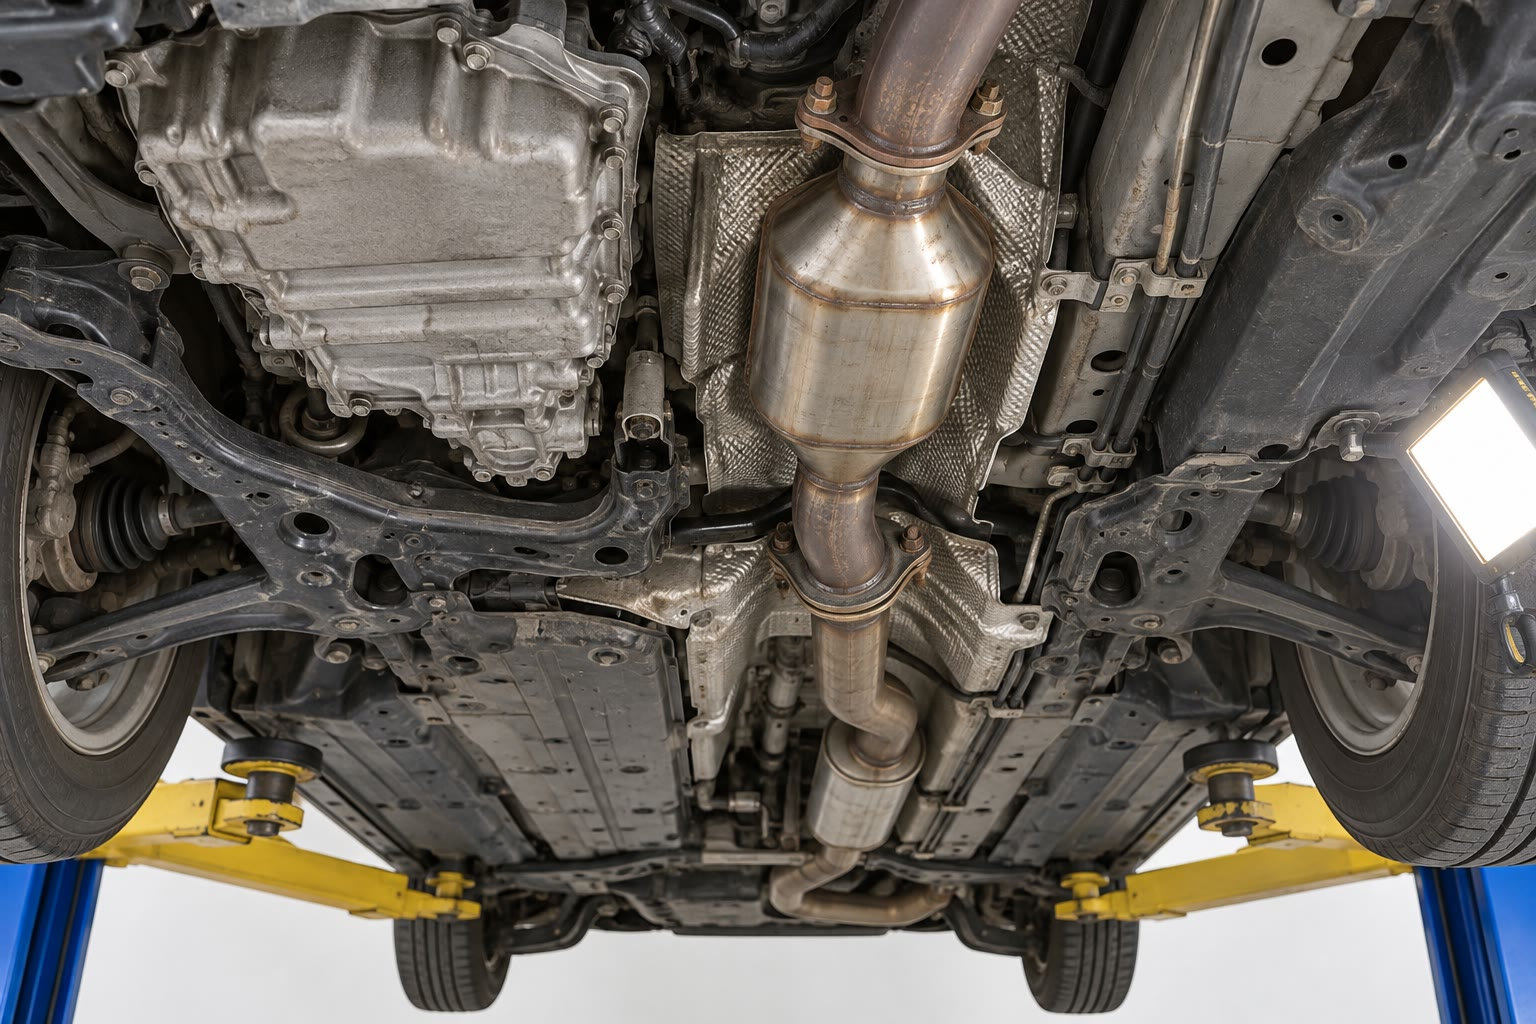
\includegraphics[width=0.5\linewidth]{images/book2/ai/b1-09-catalytic-converter.jpg}

{\small A parte de baixo de um carro: o recipiente na linha de escape é
um conversor catalítico, um \omterm{def:b1:elementary-steps:catalyst}{catalisador} heterogêneo em cuja superfície
metálica os gases de escape reagem.}
\end{omfigure}

\begin{definition}[Controle cinético e controle termodinâmico]\label{def:b1:elementary-steps:control}
Quando um reagente pode dar dois produtos por caminhos concorrentes, a
reação está sob \emph{controle cinético}\index{controle cinetico@controle cinético} se as
proporções dos produtos são fixadas pelas \omterm{def:b1:rate-laws:rate}{velocidades de formação} (o
produto de barreira mais baixa predomina), e sob \emph{controle
termodinâmico}\index{controle termodinamico@controle termodinâmico} se os caminhos são
reversíveis e o sistema atinge o equilíbrio (o produto mais estável
predomina).
\end{definition}

\begin{example}[Escolher o produto]\label{ex:b1:elementary-steps:control}
Um reagente dá B por uma barreira de \qty{50}{kJ/mol} ($\Delta E =
\qty{-10}{kJ/mol}$) e C por uma barreira de \qty{70}{kJ/mol} ($\Delta E =
\qty{-40}{kJ/mol}$). A \qty{300}{K} e em tempos curtos, com \omterm{def:b1:rate-laws:activation-energy}{fatores
pré-exponenciais} iguais, B se forma $\exp(20000/(8.314 \times 300)) \approx
3000$ vezes mais depressa que C: o \omterm{def:b1:elementary-steps:control}{controle cinético} dá B. A alta
temperatura e em tempos longos, B volta por sua pequena barreira inversa,
C não, e o sistema termina como C: \omterm{def:b1:elementary-steps:control}{controle termodinâmico}.
\end{example}

\begin{history}[A catálise, 1835]
Em 1835, o químico sueco Jöns Jacob Berzelius reuniu sob uma única
palavra uma dúzia de observações intrigantes --- o amido transformado em
açúcar pelos ácidos, o peróxido de hidrogênio decomposto pelos metais, o
álcool oxidado sobre a platina --- e chamou de ``catalítica'' a força
oculta em ação. Foi preciso a cinética do fim do século, com Wilhelm
Ostwald, para definir um \omterm{def:b1:elementary-steps:catalyst}{catalisador} como uma espécie que altera a
velocidade de uma reação, e não o seu equilíbrio.
\end{history}

\section{Exercícios}

\begin{exercise}[$\star$]\label{exo:b1:elementary-steps:1}
Dê a \omterm{def:b1:elementary-steps:elementary-step}{molecularidade} de cada etapa e diga quais etapas podem ser elementares:
(a) $\ce{N2O5 -> NO2 + NO3}$; (b) $\ce{NO + NO3 -> 2NO2}$;
(c) $\ce{2H2 + O2 -> 2H2O}$; (d) $\ce{O + O2 + N2 -> O3 + N2}$.
\end{exercise}

\begin{exercise}[$\star$]\label{exo:b1:elementary-steps:2}
Escreva a \omterm{def:b1:rate-laws:order}{lei de velocidade} das \omterm{def:b1:elementary-steps:elementary-step}{etapas elementares} $\mathrm{A} + \mathrm{B} \to
\mathrm{C}$, $2\,\mathrm{A} \to \mathrm{B}$ e $\mathrm{A} \to \mathrm{B} +
\mathrm{C}$. Por que não se pode escrever a \omterm{def:b1:rate-laws:order}{lei de velocidade} de uma
reação global a partir de sua equação?
\end{exercise}

\begin{exercise}[$\star$]\label{exo:b1:elementary-steps:3}
No \omterm{def:b1:elementary-steps:energy-profile}{perfil de energia} em duas etapas desenhado neste capítulo
(intermediário em 30, \omterm{def:b1:elementary-steps:energy-profile}{estados de transição} em 70 e 55, produtos em
$-40$, em \unit{kJ/mol} acima dos reagentes), identifique o
intermediário, os \omterm{def:b1:elementary-steps:energy-profile}{estados de transição} e a \omterm{def:b1:elementary-steps:rds}{etapa determinante da
velocidade}. A primeira etapa é endotérmica ou exotérmica?
\end{exercise}

\begin{exercise}[$\star$]\label{exo:b1:elementary-steps:4}
Um \omterm{def:b1:elementary-steps:catalyst}{catalisador} multiplica por $10^4$ a \omterm{def:b1:rate-laws:order}{constante de velocidade} direta de
uma \omterm{def:b1:elementary-steps:elementary-step}{etapa elementar}. Por quanto ele multiplica a \omterm{def:b1:rate-laws:order}{constante de velocidade}
inversa? E a constante de equilíbrio? E o tempo necessário para atingir
o equilíbrio?
\end{exercise}

\begin{exercise}[$\star\star$]\label{exo:b1:elementary-steps:5}
Para $\mathrm{A} \to \mathrm{B} \to \mathrm{C}$ com $k_1 =
\qty{0.10}{s^{-1}}$ e $k_2 = \qty{0.30}{s^{-1}}$, calcule $t_{\max}$ e a
maior concentração de $\mathrm{B}$, em unidades de $a_0$.
\end{exercise}

\begin{exercise}[$\star\star$]\label{exo:b1:elementary-steps:6}
Para $\mathrm{A} \underset{k_{-1}}{\overset{k_1}{\rightleftharpoons}}
\mathrm{I} \xrightarrow{k_2} \mathrm{P}$, com todas as etapas de ordem 1,
aplique a \omterm{def:b1:elementary-steps:qssa}{aproximação do estado estacionário} a $\mathrm{I}$ e mostre que
$v =
\frac{k_1k_2}{k_{-1} + k_2}[\mathrm{A}]$. Discuta os casos $k_2 \gg
k_{-1}$ e $k_2 \ll k_{-1}$.
\end{exercise}

\begin{exercise}[$\star\star$]\label{exo:b1:elementary-steps:7}
Os íons iodeto catalisam a decomposição do peróxido de hidrogênio:
\ce{H2O2 + I- -> H2O + IO-} (lenta), depois \ce{H2O2 + IO- -> H2O + O2 + I-}
(rápida). Escreva a equação global, identifique o \omterm{def:b1:elementary-steps:catalyst}{catalisador} e o
intermediário e dê a \omterm{def:b1:rate-laws:order}{lei de velocidade}.
\end{exercise}

\begin{exercise}[$\star\star$]\label{exo:b1:elementary-steps:8}
Uma etapa forma um carbocátion a partir de uma molécula neutra, um
processo fortemente ascendente. Usando o postulado de Hammond, explique
por que um substituinte que estabiliza o carbocátion também acelera a
etapa.
\end{exercise}

\begin{exercise}[$\star\star$]\label{exo:b1:elementary-steps:9}
No \cref{ex:b1:elementary-steps:control}, calcule a razão entre as
\omterm{def:b1:rate-laws:order}{constantes de velocidade} de formação de B e de C a \qty{300}{K} e a
\qty{600}{K}. Comente.
\end{exercise}

\begin{exercise}[$\star\star\star$]\label{exo:b1:elementary-steps:10}
Um gás $\mathrm{A}$ se decompõe depois de ser ativado por colisão com
qualquer molécula $\mathrm{M}$: $\mathrm{A} + \mathrm{M} \rightleftharpoons
\mathrm{A}^* + \mathrm{M}$ ($k_1$, $k_{-1}$), depois $\mathrm{A}^* \to
\mathrm{P}$ ($k_2$). Com a \omterm{def:b1:elementary-steps:qssa}{aproximação do estado estacionário} para
$\mathrm{A}^*$, encontre $v$ e mostre que a reação é de ordem 1 a alta
pressão e de ordem 2 a baixa pressão.
\end{exercise}

\begin{exercise}[$\star\star\star$]\label{exo:b1:elementary-steps:11}
Demonstre a fórmula de $[\mathrm{B}](t)$ do
\cref{thm:b1:elementary-steps:consecutive} e trate o caso particular
$k_1 = k_2 = k$, para o qual $[\mathrm{B}] = a_0kt\,\eu^{-kt}$.
\end{exercise}

\begin{exercise}[$\star\star\star$]\label{exo:b1:elementary-steps:12}
A reação global $\mathrm{A} + 2\,\mathrm{B} \to \mathrm{P} +
\mathrm{C}$ tem a \omterm{def:b1:rate-laws:order}{lei de velocidade} experimental $v =
k[\mathrm{A}][\mathrm{B}]^2/[\mathrm{C}]$. Proponha um mecanismo com um
pré-equilíbrio rápido que a explique.
\end{exercise}

\section{Problema: Por que o monóxido de nitrogênio se oxida mais depressa no frio}

\begin{problem}[{Problema de fim de semana --- a oxidação de terceira
ordem do monóxido de nitrogênio, um pré-equilíbrio pelo dímero
\ce{N2O2}, o tratamento do estado estacionário e uma \omterm{def:b1:rate-laws:activation-energy}{energia de ativação}
aparente negativa}]
\label{pb:b1:elementary-steps:1}
Para \ce{2NO(g) + O2(g) -> 2NO2(g)}, medidas de \omterm{def:b1:rate-laws:initial-rate}{velocidade inicial} a
\qty{300}{K} dão (velocidades em \unit{mol.L^{-1}.s^{-1}}):
\begin{center}
\begin{tabular}{cccc}
\hline
experimento & $[\ce{NO}]_0$ (mol/L) & $[\ce{O2}]_0$ (mol/L) & $v_0$ \\
\hline
1 & \num{1.0e-3} & \num{1.0e-3} & \num{1.0e-5} \\
2 & \num{2.0e-3} & \num{1.0e-3} & \num{4.0e-5} \\
3 & \num{1.0e-3} & \num{2.0e-3} & \num{2.0e-5} \\
\hline
\end{tabular}
\end{center}
A \omterm{def:b1:rate-laws:order}{constante de velocidade} encontrada a \qty{400}{K} é dez vezes menor que
a \qty{300}{K}. Considere $R = \qty{8.314}{J/(mol.K)}$.
O mecanismo proposto é
\[
  \ce{2NO <=> N2O2} \ \ (k_1, k_{-1}, \text{rápida}), \qquad
  \ce{N2O2 + O2 -> 2NO2} \ \ (k_2, \text{lenta}).
\]

\medskip
\noindent\textbf{Parte I --- A lei observada.}
\begin{enumerate}
  \item Encontre as \omterm{def:b1:rate-laws:order}{ordens parciais} em relação a \ce{NO} e a \ce{O2}.
  \item Escreva a \omterm{def:b1:rate-laws:order}{lei de velocidade} e calcule $k$ a \qty{300}{K}, com sua unidade.
  \item A reação poderia ser uma única etapa termolecular? Dê um argumento.
  \item Calcule a \omterm{def:b1:rate-laws:activation-energy}{energia de ativação} aparente a partir das duas temperaturas.
  \item Por que uma \omterm{def:b1:rate-laws:activation-energy}{energia de ativação} negativa é impossível para uma
        \omterm{def:b1:elementary-steps:elementary-step}{etapa elementar}?
  \item Escreva as \omterm{def:b1:rate-laws:rate}{velocidades de desaparecimento} de \ce{NO} e de \ce{O2}
        em função de
        $v$.
\end{enumerate}

\medskip
\noindent\textbf{Parte II --- O pré-equilíbrio.}
\begin{enumerate}[resume]
  \item Verifique que as duas etapas somadas dão a reação global. Dê o
        nome do intermediário.
  \item Dê a \omterm{def:b1:elementary-steps:elementary-step}{molecularidade} de cada etapa.
  \item Escreva a velocidade da etapa lenta.
  \item Expresse $[\ce{N2O2}]$ com a \omterm{def:b1:elementary-steps:pre-equilibrium}{aproximação do pré-equilíbrio}.
  \item Deduza a \omterm{def:b1:rate-laws:order}{lei de velocidade} e compare com o experimento.
  \item Expresse a constante observada em função de $k_1$, $k_{-1}$ e $k_2$.
\end{enumerate}

\medskip
\noindent\textbf{Parte III --- O estado estacionário.}
\begin{enumerate}[resume]
  \item Escreva $\dd[\ce{N2O2}]/\dd t$ para o mecanismo completo.
  \item Aplique a \omterm{def:b1:elementary-steps:qssa}{aproximação do estado estacionário} e expresse $[\ce{N2O2}]$.
  \item Deduza a \omterm{def:b1:rate-laws:order}{lei de velocidade} $v = \dfrac{k_1k_2[\ce{NO}]^2[\ce{O2}]}{k_{-1} +
        k_2[\ce{O2}]}$.
  \item Em que limite ela se reduz ao resultado da Parte II?
  \item Quais seriam as ordens no limite oposto?
  \item Que limite as medidas da Parte I confirmam?
\end{enumerate}

\medskip
\noindent\textbf{Parte IV --- A \omterm{def:b1:rate-laws:activation-energy}{energia de ativação} aparente.}
Cada etapa segue a \omterm{thm:b1:rate-laws:arrhenius}{lei de Arrhenius}, com \omterm{def:b1:rate-laws:activation-energy}{energias de ativação} $E_1 =
\qty{2}{kJ/mol}$, $E_{-1} = \qty{40}{kJ/mol}$ e $E_2 =
\qty{15}{kJ/mol}$.
\begin{enumerate}[resume]
  \item Escreva $\ln k$ em função dos logaritmos de $k_1$, $k_{-1}$ e
        $k_2$.
  \item Deduza $E_a = E_1 - E_{-1} + E_2$.
  \item Interprete: por que uma combinação de \omterm{def:b1:elementary-steps:elementary-step}{etapas elementares} pode ter
        uma \omterm{def:b1:rate-laws:activation-energy}{energia de ativação} aparente negativa?
  \item Esboce o \omterm{def:b1:elementary-steps:energy-profile}{perfil de energia}: onde fica o segundo \omterm{def:b1:elementary-steps:energy-profile}{estado de
        transição}, em relação aos reagentes \ce{2NO + O2}?
  \item Por qual fator a velocidade variaria entre 300 e \qty{400}{K}
        com esse valor?
  \item Calcule a \omterm{def:b1:rate-laws:activation-energy}{energia de ativação} aparente a partir dos valores das
        etapas e compare com a Parte I.
\end{enumerate}
\end{problem}
